\documentclass[../teoria.root.tex]{subfiles}

\begin{document}

\section{Planos}

En $\mathbb{R}^2$, una recta se puede definir, dado un punto $P$ en la recta y
un vector perpendicular $N$, como el conjunto de puntos $X$ donde el vector
$\vec{PX}$ sea perpendicular a $N$:
\[\{X\in\mathbb{R}^2:(X-P)\cdot N=0\}\]

\begin{center}
	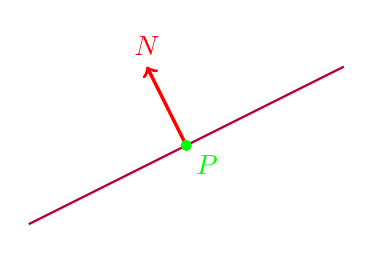
\begin{tikzpicture}
		\draw[purple,thick] (-2,-1) -- (2,1);
		\draw[red,->,very thick] (0,0) -- (-.5,1) node[above]{$N$};
		\fill[green] circle(2pt) node[below right]{$P$};
	\end{tikzpicture}
\end{center}

Al extender este concepto a $\mathbb{R}^3$, el conjunto resultante va a
representar un plano:
\[\{X\in\mathbb{R}^3:(X-P)\cdot N=0\}\]

\begin{center}
	\tdplotsetmaincoords{120}{250}
	\begin{tikzpicture}[tdplot_main_coords]
		\plane{-1}{1}{1}{0}{2}{purple};
		\draw[red,->,very thick] (0,0,0) -- (-1,1,1) node[above]{$N$};
		\fill[green] circle(2pt) node[above right]{$P$};
	\end{tikzpicture}
\end{center}

\subsection{Ecuación implícita}

Al igual que con las rectas, esta representación se puede transformar en una
ecuación implícita. Por ejemplo, la ecuación del plano que pasa por $(3,-1,2)$
con vector normal $(1,-2,4)$ seria:
\begin{align*}
	(X-P)\cdot N&=0\\
	X\cdot N&=P\cdot N\\
	(x,y,z)\cdot(1,-2,4)&=(3,-1,2)\cdot(1,-2,4)\\
	x-2y+4z&=13
\end{align*}

Resumiendo, dados un vector $N=(a,b,c)$ y un punto $P$, el plano $\Pi$
perpendicular a $N$ y que pasa por $P$ sería:
\begin{align*}
	\Pi&=\{X\in\mathbb{R}^3:X\cdot N=P\cdot N\}\\
	&=\{(x,y,z)\in\mathbb{R}^3:ax+by+cz=d\}\tag{con $d=P\cdot N$}
\end{align*}

Y en notación abreviada:
\[\Pi:ax+by+cz=d\]

\subsection{Plano que pasa por 3 puntos}

Al igual que una recta se puede definir mediante dos puntos sobre la misma, un
plano se puede definir con tres puntos, siempre y cuando no estén alineados.
Podemos utilizar cualquiera de los puntos como $P$, pero nos faltaría encontrar
un vector normal al plano. Por suerte, el producto vectorial de dos vectores
nos puede dar uno, así que solo tenemos que hacer $\vec{AB}\times\vec{AC}$ para
encontrarlo. Por ejemplo, para encontrar la ecuación de un plano $\Pi$ que pasa
por los puntos $A=(1,2,1)$, $B=(-2,3,1)$ y $C=(0,1,3)$:
\begin{gather*}
	\begin{split}
		N&=(B-A)\times(C-A)\\
		&=(-3,1,0)\times(-1,-1,2)\\
		&=(2,6,4)
	\end{split}\\
	A\cdot N=(1,2,1)\cdot(2,6,4)=18\\
	\Pi:2x+6y+4z=18
\end{gather*}

\begin{center}
	\begin{tikzpicture}[tdplot_main_coords]
		\plane[(0,1)]{2}{6}{4}{18}{3}{purple};
		\coordinate (a) at (1,2,1);
		\coordinate (b) at (-2,3,1);
		\coordinate (c) at (0,1,3);
		\draw[red,->,very thick] (a) -- (b);
		\draw[green,->,very thick] (a) -- (c);
		\draw[blue,->,very thick] (a) -- ++(0.8,2.4,1.6) node[above]{$N$};
		\fill (a) circle(2pt) node[right]{$A$};
		\fill (b) circle(2pt) node[left]{$B$};
		\fill (c) circle(2pt) node[left]{$C$};
	\end{tikzpicture}
\end{center}

\subsubsection{Puntos alineados}

¿Cómo sabemos si tres puntos $A$ $B$ y $C$ forman parte de una misma recta? La
solución es simple: Para que los tres puntos formen parte de la misma recta, la
recta que pasa entre $A$ y $B$ debe ser igual a la que pasa por $A$ y $C$, osea
que sus vectores directores, $\vec{AB}$ y $\vec{AC}$ sean paralelos, osea que
sean múltiplos:
\[\{A,B,C\}\subset\mathbb{L}\iff\vec{AB}\parallel\vec{AC}\iff\exists k:B-A=k(C-A)\]

Si los puntos están alineados, este procedimiento para encontrar un plano no
funciona, ya que conseguiríamos $\vec{AB}\times\vec{AC}=(0,0,0)$, que no
podemos usar como vector normal. Cuando los puntos están alineados, el problema
se reduce a buscar un plano que pase por una recta.

\subsection{Plano que pasa por una recta}

No existe un solo plano que pase por una recta, sino que hay infinitos, así que
tenemos que elegir uno. Cualquier vector normal de uno de los posibles planos
también va a ser normal a la recta. Podemos utilizar esta propiedad para
resolver la ecuación $N\perp\vec{v}$. Por ejemplo, con la recta que pasa por
los puntos $A=(2,3,3)$ y $B=(0,-1,-3)$:
\begin{align*}
	N\cdot(B-A)&=0\\
	(a,b,c)\cdot((0,-1,-3)-(2,3,3))&=0\\
	(a,b,c)\cdot(-2,-4,-6)&=0\\
	-2a-4b-6c&=0
\end{align*}

Esta ecuación nos va a dar todos los posibles vectores normales de un plano que
pase por la recta. Ahora reemplazamos dos de las incógnitas por los valores que
se nos cante, y despejamos la que quede para conseguir el vector normal:
\begin{gather*}
	\begin{split}
		a=b&=1\\
		-2-4-6c&=0\\
		c&=-1\\
		N&=(1,1,-1)
	\end{split}\\
	A\cdot N=2\\
	\Pi:x+y-z=2
\end{gather*}

% Este no es realmente el plano del problema, pero se ve mas claro
\begin{center}
	\begin{tikzpicture}[tdplot_main_coords]
		\plane{1}{0}{1}{0}{3}{purple};
		\coordinate (a) at (0,3.5,0);
		\coordinate (b) at (0,-3.5,0);
		\draw[red, very thick] (a) -- (b);
		\fill (a) circle(2pt) node[right]{$A$};
		\fill (b) circle(2pt) node[left]{$B$};
	\end{tikzpicture}
\end{center}

\subsection{Ecuación paramétrica}

La ecuación implícita de un plano es una condición que debe cumplir un punto
para pertenecer al mismo, pero al igual que las rectas, existe una ecuación
paramétrica, en la que se reemplazan parámetros para conseguir puntos.

Tomemos por ejemplo el plano $\Pi:2x+3y-z=7$, podemos despejar una de las
incógnitas y terminar con una ecuación de dos términos:
\begin{gather*}
	2x+3y-z=7\\
	z=2x+3y-7\\
	X=(x,y,z)\in\Pi\iff X=(x,y,2x+3y-7)\\
	\Pi=\{(x,y,2x+3y-7)\forall x,y\in\mathbb{R}\}
\end{gather*}

Esta ecuación depende únicamente de $x$ e $y$. Podemos limpiar un poco la
ecuación separando los términos con $x$, $y$ y los términos sin variables:
\begin{align*}
	X&=(\mcol{x}{x},\mcol{y}{y},\mcol{x}{2x}\mcol{y}{+3y}\mcol{z}{-7})\\
	&=\mcol{x}{x(1,0,2)}+\mcol{y}{y(0,1,3)}+\mcol{z}{(0,0,-7)}
\end{align*}

Lo que tenemos ahora se parece mucho a la ecuación paramétrica de una recta,
pero con dos parámetros. Esta es la ecuación paramétrica de un plano.
\[\Pi:X=\alpha\vec{v}+\beta\vec{w}+P\]

Los vectores $\vec{v}$ y $\vec{w}$ son los vectores directores de dos rectas
paralelas al plano. Para pasar de ecuación paramétrica a implícita se puede
conseguir un vector normal haciendo $\vec{v}\times\vwc{w}$.

\subsection{Intersecciones}

\subsubsection{Entre plano y recta}

La intersección entre una linea $\mathbb{L}$ y un plano $\Pi$ se puede
conseguir con el siguiente procedimiento, ilustrado con un ejemplo:
\begin{gather*}
	\mathbb{L}:\lambda(1,1,2)+(-3,1,4)\\
	\Pi:2x+3z=2
	\intertext{El conjunto $Q$ va a ser la intersección del plano y la recta:}
	\begin{split}
		Q=(x,y,z)\in\mathbb{L}\cap\Pi\iff&\exists\lambda:\lambda(1,1,2)+(-3,1,4)\\
		&\land 2x+3z=2
	\end{split}
	\intertext{Primero se aplica la ecuación de la recta:}
	\begin{split}
		\lambda(1,1,2)+(-3,1,4)&=(\lambda,\lambda,2\lambda)+(-3,1,4)\\
		&=(\lambda-3,\lambda+1,2\lambda+4)
	\end{split}
	\intertext{Luego se reemplaza el punto en la ecuación del plano para despejar $\lambda$:}
	\begin{split}
		2(\lambda-3)+3(2\lambda+4)&=2\\
		2\lambda-6+6\lambda+12&=2\\
		8\lambda&=-4\\
		\lambda&=-\frac{1}{2}
	\end{split}
	\intertext{Y finalmente se reemplaza $\lambda$ en la ecuación de la recta:}
	\begin{split}
		\lambda(1,1,2)+(-3,1,4)&=-\frac{1}{2}(1,1,2)+(-3,1,4)\\
		&=\left(-\frac{1}{2},-\frac{1}{2},-1\right)+(-3,1,4)\\
		&=\left(-\frac{7}{2},\frac{1}{2},3\right)\\
	\end{split}
\end{gather*}

\begin{center}
	\begin{tikzpicture}[tdplot_main_coords]
		\coordinate (p) at (-7/2,1/2,3);
		\draw[red,thick] (p) -- ++(-1,-1,-2);
		\plane[(-4.5,0)]{2}{0}{3}{2}{2}{purple};
		\draw[red,thick] (p) -- ++(1,1,2);
		\fill[green] (p) circle(2pt);
	\end{tikzpicture}
\end{center}

Podría pasar que al reemplazar en la ecuación del plano se cancelen todas las
incógnitas, en cuyo caso la recta forma parte del plano. También podríamos
haber llegado a una contradicción, en cuyo caso la recta y el plano no se
tocan.

\subsubsection{Entre planos}

Calcular la intersección entre dos planos es básicamente resolver un sistema de
ecuaciones. Por ejemplo, dados los planos $\Pi_1:2x+y+2z=4$ y $\Pi_2:x-y+3z=5$:
\begin{gather*}
	\begin{align*}
		&\systeme{2x+y+2z=4,x-y+3z=5}&&\to
		&&\begin{cases}y=4-2x-2z\\x-y+3z=5\end{cases}&&\to\\
		&\begin{cases}y=4-2x-2z\\x-(4-2x-2z)+3z=5\end{cases}&&\to
		&&\begin{cases}y=4-2x-2z\\x=3-\frac{5}{3}z\end{cases}&&\to\\
		&\begin{cases}y=4-2\left(3-\frac{5}{3}z\right)-2z\\x=3-\frac{5}{3}z\end{cases}&&\to
		&&\begin{cases}y=-2+\frac{4}{3}z\\x=3-\frac{5}{3}z\end{cases}
	\end{align*}\\
	\begin{split}
		X=(x,y,z)&=\left(3-\frac{5}{3}z,-2+\frac{4}{3}z,z\right)\\
		&=z\left(-\frac{5}{3},\frac{4}{3},1\right)+(3,-2,0)
	\end{split}
\end{gather*}

Terminamos con la ecuación paramétrica de una recta, equivalente a la
intersección de los dos planos.
\begin{center}
	\tdplotsetmaincoords{135}{15}
	\begin{tikzpicture}[tdplot_main_coords]
		\plane{2}{1}{2}{4}{3}{red};
		\plane{1}{-1}{3}{5}{3}{green};
		\coordinate (p) at (3,-2,0);
		\coordinate (z) at (-5/3,4/3,1);
		\draw[dashed,very thick,purple] ($(p)-.5*(z)$) -- ($(p)+3.5*(z)$);
	\end{tikzpicture}
\end{center}

Podría pasar que al reemplazar en la ecuación del plano se cancelen todas las
incógnitas, en cuyo caso las dos ecuaciones describen el mismo plano. También
podríamos haber llegado a una contradicción, en cuyo caso los planos no se
tocan.

\subsection{Distancia de punto a plano}

La distancia de un punto $P$ a un plano $\Pi$ va a ser la distancia entre $P$ y
el punto mas cercano de $\Pi$, así que para calcular la distancia vamos a tener
que encontrar ese punto. El punto mas cercano va a ser aquel que forme parte de
una recta $\mathbb{L}$ perpendicular a $\Pi$ que pase por el punto
$P$.\footnote{¿Por qué? Llamemos $R$ al punto que esta sobre $\mathbb{L}$. Si
tomamos cualquier otro punto en el plano, llamémoslo $Q$, este va a formar un
triangulo rectángulo $PRQ$. El segmento $\overline{PQ}$ es la hipotenusa del
triangulo, y por lo tanto mas largo que el cateto $\overline{RP}$.}

$\mathbb{L}$ es fácil de conseguir. Su vector director va a ser el mismo que el
vector normal del plano, y $P$ nos sirve como punto de paso. Luego solo falta
encontrar $\mathbb{L}\cap\Pi$, y calcular la distancia al punto resultante.

Por ejemplo, con el plano $\Pi:-x+y+4z=10$ y el punto $P=(1,-3,8)$:
\begin{gather*}
	\mathbb{L}:\lambda(-1,1,4)+(1,-3,8)\\
	R\in\mathbb{L}\cap\Pi\\
	R=(x,y,z)=\lambda(-1,1,4)+(1,-3,8)=(-\lambda+1,\lambda-3,4\lambda+8)\\
	\begin{align*}
		-x+y+4z&=10\\
		-(-\lambda+1)+(\lambda-3)+4(4\lambda+8)&=10\\
		\lambda-1+\lambda-3+16\lambda+32&=10\\
		18\lambda&=-18\\
		\lambda&=-1
	\end{align*}\\
	R=\lambda(-1,1,4)+(1,-3,8)=(1,-1,-4)+(1,-3,8)=(2,-4,4)
\end{gather*}

\end{document}
